% ****** Start of file aipsamp.tex ******
%
%   This file is part of the AIP files in the AIP distribution for REVTeX 4.
%   Version 4.1 of REVTeX, October 2009
%
%   Copyright (c) 2009 American Institute of Physics.
%
%   See the AIP README file for restrictions and more information.
%
% TeX'ing this file requires that you have AMS-LaTeX 2.0 installed
% as well as the rest of the prerequisites for REVTeX 4.1
%
% It also requires running BibTeX. The commands are as follows:
%
%  1)  latex  aipsamp
%  2)  bibtex aipsamp
%  3)  latex  aipsamp
%  4)  latex  aipsamp
%
% Use this file as a source of example code for your aip document.
% Use the file aiptemplate.tex as a template for your document.
\documentclass[aip,nobalancelastpage,
twocolumn,
%sd,%
rsi,%
 amsmath,amssymb,
%preprint,%
 reprint,%
%author-year,%
%author-numerical,%
]{revtex4}

\usepackage{float}
\usepackage{amsfonts}
\usepackage[]{algorithmic}
\usepackage{graphicx}% Include figure files
\usepackage{dcolumn}% Align table columns on decimal point
\usepackage{listings}
\usepackage[utf8]{inputenc}
\usepackage[norsk]{babel}
\usepackage{bm}% bold math
\usepackage{verbatim}
\usepackage{hyperref}
\usepackage{xcolor}

%\usepackage[mathlines]{lineno}% Enable numbering of text and display math
%\linenumbers\relax % Commence numbering lines



\begin{document}

\preprint{AIP/123-QED}

\title{Project 2: Writing an Eigenvalue Solver which can be applied to Scaled Differential Equations}

\author{Noah Oldfield}

\affiliation{ 
Department of physics, University of Oslo%\\This line break forced with \textbackslash\textbackslash
}%

\date{\today}% It is always \today, today,
             %  but any date may be explicitly specified

\begin{abstract}
In this report, we write a numerical eigenvalue solver using Jacobi's eigenvalue algorithm. We see how this solver can be applied to widely different physical systems when proper scaling of differential equations are made. There are three parts: in part 1 we study a buckling beam system, where we compare the computed eigenvalues of the solver with known analytical values. We then test the computed values towards the numpy.linalg.eig solver and find that the values hold up to a specific set precision. The runtimes of the two however greatly favour the written solver. In part 2 we study a quantum system in a spherical symmetric potential, we find that we can reuse our solver by simply adding the potential values to the diagonal of our matrix. In addition we find that $\rho_N=10$ is a decent approximation to infinity for the quantum system, resulting in an error (between computed and analytical energy values) which tends to zero for a $(N \times N)$ matrix. In part 3 we study two electrons with a repulsion force and also in spherical symmetric potential, so called quantum dots. We study the ground state energy eigenvalues, which are proportional to the computed eigenvalues, and find that an increase in the potential strength leads to an increase in the seperation of the electrons.

\end{abstract}

\keywords{Suggested keywords}%Use showkeys class option if keyword
                              %display desired
\maketitle

Github repository: \url{https://github.com/nhofield/fys3150Projects.git} 

\section{Introduction}

In this report we will use Jacobi's eigenvalue algorithm to write a common solver for three seemingly different physical systems. There are three parts: part 1-3 centers on a buckling beam system, a particle in spherically symmetrical potential and two electrons with a repulsion force respectively. Each will be shown solvable by the same solver by only adding elements to the diagonal of our matrix $A$ custom to each system.\par
The solver will use Jacobi's eigenvalue algorithm to solve for the eigenvalues of a symmetric matrix $A$, and unit tests will be implemented in order to test mathematical properties of the algorithm and other functions in the program. There are great advantages when it comes to implementing unit tests during the development phase in light of debugging. Especially when the programs become relatively large and complex such as in this case.\par

\section{Theory}
\subsection{Unitary Transformations}
Let $v_i^T = (v_{i1},v_{i2},\cdots, v_{in})$ where n=1,2,3,.. be an orthonormal vector from some orthonormal basis of dimension $n$; and let U be a unitary or orthogonal matrix.\par
A unitary or orthogonal transformation $\hat{w}_i = U\hat{v}_i$ is a transformation such that the orthonormality of a specific basis is preserved. \par
\subsubsection{Proof}
We'll consider another basisvector from the same basis of $\hat{v}_i$, $\hat{v}_j$ and both are considered to have real inputs. The inner product between $\hat{v}_i$ and $\hat{v}_j$ is assumed equal to the matrix product of $v_i^T$ with $\hat{v}_j$ denoted 
\begin{equation}
\left<\hat{v}_i, \hat{v}_j \right> = v_i^T\hat{v}_j
\end{equation}
thus the inner product of the unitary or orthogonal transformations is 
\begin{equation}
\left<\hat{w}_i,\hat{w}_j\right> = w_i^T\hat{w}_j=\left(U\hat{v_i}\right)^TU\hat{v}_j = v_i^TU^TU\hat{v}_j
\end{equation}
since U is real orthogonal and using the associative property, then $(U^T U) = I$, where $I$ denotes the identity matrix. Thus
\begin{equation}
\left<\hat{w}_i,\hat{w}_j\right> = v_i^T \hat{v}_j=\left<\hat{v}_i,\hat{v}_j\right>
\end{equation}
Furthermore, since both $\hat{v}_i$ and $\hat{v}_j$ are elements of the same orthonormal basis, the inner product is equal to the Kronecker-delta
\begin{equation}
\left<\hat{w}_i,\hat{w}_j\right> =\left<\hat{v}_i,\hat{v}_j\right> = \delta_{ij}
\end{equation}
which equates to zero for $i\neq j$ and $1$ for $i=j$. Thus preserving the orthonormality.\par
In order to prove the same for a unitary transformation one must make a similar assumption with the inner
product between two complex vectors $\left<\hat{v}_i, \hat{v}_j\right> = \hat{v}_i^\dagger \hat{v}_j$ and use the unitary condition $U^\dagger U = I$ instead. Thus proving orthonormality in this case also.\par
Thus it would seem that unitary transformations preserve orthonormality for both real and complex bases, but the orthogonal transformations do not necessarily preserve orthonormality for complex bases.
QED

\subsection{Scaled differential Equations}

\subsubsection{Part 1: Buckling-Beam problem}
The differential equation
\begin{equation}
\gamma \frac{d^2 u(x)}{dx^2}=-F u(x)
\end{equation}
describes a vertically oscillating buckling beam of length $L$ due to its rigidity $\gamma$ and force F which acts to perpetually return the beam to equilibrium. The equation will be solved using Dirichlet boundary conditions over the discretized values of x$\in [0, L]$ meaning the first and last values of x yields $u(L)=u(0)=0$.\par
By introducing a dimensionless parameter $\rho = \frac{x}{L}$ the differential equation reduces to the following dimensionless equation
\begin{equation}
\frac{d^2 u(\rho)}{d\rho^2}=-\frac{FL^2}{R}u(\rho)=-\lambda u(\rho)
\end{equation}
with the $\rho \in [0,1]$ and $u(0)=u(1)=0$ due to the definition of $\rho$.

\subsubsection{Part 2: Schrodinger-Equation}
Now introducing the Schrodinger equation for a particle in a spherical symmetric potential $V(r)$
\begin{equation}
-\frac{\hbar^2}{2m}\left(\frac{1}{r^2}\frac{d}{dr}r^2\frac{d}{dr}-\frac{l(l+1)}{r^2}\right)R(r)+V(r)R(r)=E R(r)
\end{equation} 
We'll take the potential to be the harmonic oscillator potential $V(r)=\frac{1}{2}k r^2$ where $k=m\omega^2$.
The same procedure can be followed to scale the equation, though slightly more sofisticated. We begin by introducing two dimensionless variables $R(r)=\frac{u(r)}{r}$ and $\rho(r)=\frac{r}{\alpha}$ which turns out to simplify certain terms in the radial Schrodinger equation which come from the laplacian operator $\nabla^2$ in spherical coordinates.
The first step is to compute 
\begin{equation}
\left(\frac{1}{r^2}\frac{d}{dr}r^2\frac{d}{dr}\right) \frac{u(r)}{r}
\end{equation}
and following the algebra from this and inserting the potential $V(r)=\frac{1}{2}k r^2$ one can arrive at the equation

\begin{equation}
-\frac{d^2}{d\rho^2}u(\rho) + \frac{mk}{\hbar^2}\alpha^4 \rho^2 u(\rho)=\frac{2m\alpha^2}{\hbar^2}Eu(\rho)
\end{equation}
Now we can fix either of the constants on the left side in front of either the double derivative term or the other to 1. The purpose of the scaling is to reduce the problem to a general form of differential equation which can then be solved using a particular numerical solver.
By choosing to fix the second term on the left side to 1 the equation reduces to the dimensionless differential equation
\begin{equation}
-\frac{d^2}{d\rho^2}u(\rho) +\rho^2 u(\rho) = \lambda u(\rho)
\end{equation}

\subsubsection{Part 3: Quantum-dots in 3 dimensions}
We shall also be making computations for a system of two electrons in a harmonic oscillator potential which also interact through a repulsive Coulomb interaction. We shall not go into detail for the scaling of this equation, but simply post the differential equation and define all terms.
\begin{equation}
\label{theory-quantumdotsdiffeq}
-\frac{d^2}{d\rho^2}\psi(\rho) + \omega_r^2 \rho^2\psi(\rho) + \frac{1}{\rho} = \lambda \psi(\rho)
\end{equation}
The equation is scaled such that $\rho = \frac{r}{\alpha}$ where $\alpha$ is a length reference parameter. The parameter $\omega_r$ represents the strength of the harmonic oscillator potential and shall take on the values [0.01, 0.5, 5]. The coordinate $r$ and thereby $\rho$ in this case represents the relative distance between the electrons.

\subsection{Analytical solutions and other definitions}

\subsubsection{Analytical Eigenvalues for the Buckling Beam Toeplitz Matrix}
The eigenvalues for the coming $(N\times N)$ matrix $A$, given by the finite difference method for the buckling beam problem, are given by
\begin{equation}
\label{AnalyticalBucklingEigenvals}
\lambda_j = d + 2a\cos\left(\frac{j \pi}{N+1}\right)\;\;\;\;for\; j =1,2,\cdots,N-1
\end{equation}
where $d$ are the diagonal elements of $A$ and $a$ are the just above and just below diagonal elements of $A$.

\subsubsection{Analytical Energy values for particle in spherical symmetrical potential with no orbital angular momentum}

\begin{equation}
E_n = \hbar \omega \left(2n + \frac{3}{2}\right)\;\;\;\; n=0,1,2,\cdots
\label{Energyval-Analytical}
\end{equation}
where $\hbar$ is the reduced Planck constant and $\omega$ is the angular frequency.

\subsubsection{Frobenius Norm}
The frobenius norm of a ($m\times n$) matrix $A$ is denoted $\left|\left|A\right|\right|_F$
\begin{equation}
\left|\left|A\right|\right|_F = \sqrt{\sum_{i=1}^m \sum_{j=1}^n \left|a_{ij}\right|^2}
\end{equation}
where $a_{ij}$ are the matrix elements of $A$.
\section{Numerical Method}
\subsection{Jacobi's Eigenvalue Algorithm}
The Jacobi Eigenvalue Algorithm is a means to compute the eigenvalues of a symmetric matrix $A$ by applying a sequence of orthogonal rotation transformations $J^TAJ$ until, in theory, the off diagonal elements of the resulting transformation are all zero. Thus resulting in a diagonalization with the resulting matrix being a diagonal matrix with the eigenvalues of $A$ as it's diagonal elements.\par
In short, first the largest off diagonal element is chosen (which is due to being the most efficient way of zeroing out the off diagonals), the indices of the chosen element then defines a specific Givens rotation matrix, represented by $J$.
Which the elements of are then to be calculated by 
\begin{equation}
\tau = \frac{a_{ll}-a_{kk}}{2a_{kl}}
\end{equation}
where the indices $l,k$ refer to the absolute value of the largest non diagonal element in $A$ as explained above. This helps us define and
solve the quadratic equation
\begin{equation}
\tan^2\theta +2\tau \tan\theta - 1 = 0
\end{equation}
where the solutions are given by 
\begin{equation}
t = -\tau \pm \sqrt{1+ \tau^2}
\end{equation}
and now $t=\tan\theta$ is a common shorthand notation. With this, the angle for the rotation matrix is known and the orthogonal transformation can be computed.\par
This process is repeated iteratively until the Frobenius norm of the off diagonal elements is smaller than a fixed tolerance.\par
So how many rotations are typically needed?\par 
Since the algorithm is based on zeroing out non diagonal elements in order to diagonalize the matrix, it should be safe to presume that at least $N^2 - N$ rotations for a matrix of size $(N \times N)$ are needed. But generally the orthogonal transformations often make previously zeroed out off diagonal elements non zero again at various iterations. So more than $N^2-N$ rotations are required. In lack of more information, this additional term is assumed to be $(N^2-N)/2$ or in other words at least half of the already zeroed out off diagonal elements have to be zeroed out again. This gives us a net expected number of rotations $N_{rot}(N)$ required for a $(N \times N)$ matrix 
 \begin{equation}
 \label{numberofRotequation}
 N_{rot}(N) = \frac{3}{2}N ( N-1)
 \end{equation}
so for example a $(10 \times 10)$ matrix would require $N_{rot}(10) = 165$ rotations.
\subsection{The finite difference method}
The second order derivative of a function can be approximated by
\begin{equation}
u'' = -\frac{u_{i+1} - 2u_i + u_{i-1}}{h^2}
\end{equation}
where $h$ is the chosen step length.

\subsection{Discretization}
By discretizing our differential equations and using the finite difference method, we can solve both equations by matrix equations of the form
\begin{equation}
\label{eigenvalueequation}
A\hat{u} = \lambda \hat{u}
\end{equation}
with the product $A\hat{u}$ defines the set of linear equations generated by the finite difference method. By making $A$ a general Toeplitz matrix we can write $A$ as $(N\times N)$ with the elements $d_i,b_i,c_i$
\begin{equation}
A = \begin{pmatrix}
d_1 & b_1 & 0   & 0 &   \cdots & 0 & 0 \\ 
c_1 & d_2 & b_2 & 0 & \cdots & 0 & 0 \\
0   & c_2 & d_3 & b_3 & \cdots & 0 & 0\\
  \vdots  &  \vdots   & \vdots &  &    \ddots    & \vdots & \vdots\\
0 & 0 & 0 & \cdots & c_{N-2} & d_{N-1} & b_{N-1} \\
0 & 0 & 0 & \cdots  & 0 & c_{N-1} & d_N  
\end{pmatrix}
\end{equation}
In simplicity, (\ref{eigenvalueequation}) is an eigenvalue problem. Where $\hat{u}$ is a specific eigenvector (a solution to the equation) for a specific eigenvalue (set of constants) for our problem. Physically these represent different energy states of either the buckling beam system or the quantum system.\par
Discretizing the dimensionless parameter $\rho \rightarrow \rho_i$ giving $u(\rho)\rightarrow u(\rho_i)=u_i$ and for the buckling beam $\rho_i \in [0, \frac{L}{L}]=[0,1]$ due to how we defined $\rho$.\par
The quantum system is a little bit more tricky, due to the fact that for a particle in spherical symmetric potential, $r$ runs from zero to inifinity. Since we can not define infinity, we'll have to approximate it. We'll use 1-10 as a starting points due to the small scales of quantum systems. We can choose $\rho$ to be in units of Ångstrøms [Å], where 1Å=0.1nm.\par
The matrix $A$ becomes tridiagonal due to the finite difference method and we'll define the diagonal elements as $d_i$ (i=1,2,...,N) and the diagonals above and below the main diagonal as $b_i$ and $c_i$ (i=1,2,...N-1) respectively.\par

The buckling beam problem solutions are given by
\begin{equation}
\lambda u_i = -\frac{u_{i-1} -2u_i + u_i{i+1}}{h^2}
\end{equation}
while the quantum systems has an extra term due to the potential $\rho^2u(\rho)$ which discretizes to
\begin{equation}
\lambda u_i = -\frac{u_{i-1} -2u_i + u_i{i+1}}{h^2} + \rho_i^2 u_i
\end{equation}
considering that the indices $i$ refer to the main diagonal of the matrix $A$ we see that the eigenvalue problem of the quantum system is the same as for the buckling beam except that we need to add the values of the potential to the main diagonal of $A$. The same goes for the terms in the system of two electrons ($\ref{theory-quantumdotsdiffeq}$), except the extra term becomes
\begin{equation}
\omega_r^2 \rho_i^2 u_i + \frac{1}{\rho_i}
\end{equation}
where $\omega_r$ is taken to represent the strength of the harmonic oscillator potential which the electrons are trapped within.\par
In order to make a general solver for similar equations such as this. A function which creates a Toeplitz matrix given an array of diagonal, above and below diagonal seems to be suitable. By using dynamic array allocations, the arrays for these diagonals are only needed in runtime very briefly.\par


\subsection{Program Structure and Computations}
This part describes firstly the program structure and secondly the computations which will be performed in this report.\par
The program for this computation will be written in terms of a hierarchy of functions, where a main function $JacobiEigenValueAlgorithm$ will be depend on several other functions (which in turn represent steps in the Jacobi eigenvalue algorithm). This hierarchy of functions is compactly collected in the $JacobiEigenvalSolver.h$ file.\par
The function hierarchy is divided into four function: 
\begin{itemize}
\item 1 - Calculate value of maximum off diagonal element in matrix A $\rightarrow$ function $Max\_Off\_Diag\_Element$
\item 2 - Find indices (k,l) of maximum element in the matrix A $\rightarrow$ function $Max\_Off\_Diag\_kl$
\item 3 - Perform Jacobi rotation $\rightarrow$ function $JacobiRotation$
\item 4 - Perform orthogonal matrix transformation $\rightarrow$ function $Update\_A$
\end{itemize}
all implemented in function $JacobiEigenValueAlgorithm$:

\subsection{Main Algorithm}

\begin{algorithmic}[H]
 \WHILE{$max|a_{ij}| > tol$}
 \IF{Orthogonality-Test = False}
 \STATE   {Break and print message}
\ELSE
 \STATE {Perform Jacobi rotation}
  \STATE {Perform orthogonal transformation} 
  \STATE {Update A} 
  \ENDIF
 \ENDWHILE 
\end{algorithmic}

\subsection{Unit tests}
Since our program consists of a large number of statements, functions and variables. It is a good idea to implement test functions so as to firstly confirm that the function runs as expected when initially written. And secondly to make sure it keeps executing as expected in the program.\par
Test functions are written for functions 1-3 and the main algorithm function $JacobiEigenValueAlgorithm$. The latter includes a test case for the matrix
\begin{equation}
\begin{pmatrix}
\phantom{-}1 & \phantom{-}1 & -2 \\ \phantom{-}1 & \phantom{-}2 & \phantom{-}1 \\ -2 & \phantom{-}1 & -1
\end{pmatrix}
\end{equation}
with the analytical eigenvalues $(2,\pm \sqrt{7})$.
\subsection{Other test functions}
One particularly useful function written in the program is the $CompareEigenvalueComputations$ function, which takes two arrays as inputs where each contains the analytical eigenvalues (calculated by (\ref{AnalyticalBucklingEigenvals})) and the eigenvalues computed by the Jacobi algorithm.\par
Since the order of the eigenvalues in the arrays can be somewhat random, the function compares all values and increments a counter by +1 if it finds a match. Lastly the program checks whether the counter is equal to the length of either of the received arrays. If the check is successful within a certain tolerance, the eigenvalues are considered equal. 

\subsection{About repository and programs}
There are three c++ programs 
\begin{itemize}
\item Part 1 \textit{JacobiEigenvalSolverBuck.cpp}
\item Part 2 \textit{JacobiEigenvalSolverSchr.cpp}
\item Part 3 \textit{JacobiEigenvalSolverQdots.cpp}
\end{itemize}
which are all linked to the header \textit{JacobiEigenvalSolver.h}. In addition there are corresponding python programs
\begin{itemize}
\item Part 1 \textit{JacobiEigenvalSolverNumpy.py}
\item Part 2 \textit{SchrPython.py}
\item Part 3 \textit{QdotsPython.py}
\end{itemize}
which produce the various results used in the report. There are also corresponding dat for storing the results of the c++ programs.
\section{Results}
\subsection{Part 1: Buckling-Beam problem, comparison of eigenvalues computed by Jacobi algorithm and numpy.linalg.eig}
The programs $JacobiEigenvalSolverBuck.cpp$ and $JacobiEigenvalSolverNumpy.py$ are run. Each write their own dat file $eigenvalues.dat$ and $eigenvaluespython.dat$ respectively. The values are collected from one execution and computation times logged for a series of 5 executions.

\begin{table}[H]
\caption{Table of computed eigenvalues with both Jacobi algorithm and numpy.linalg.eig function for a $(N=8 \times N=8)$ matrix $A$}

\begin{tabular}{|c|c | c |}
\hline
$\lambda_i$ & Jacobi Algorithm & numpy.linalg.eig \\
\hline
1 & 192 & 192.000000 \\
\hline
2 & 64 & 64.000000 \\
\hline
3 & 248.28066 &  248.280655 \\
\hline
4 & 7.7193445  & 7.719345  \\
\hline
5 & 150.22697 & 150.226967 \\
\hline
6 & 105.77303  & 105.773033 \\
\hline
7 & 226.05369 & 226.053689 \\
\hline
8 & 29.946311 & 29.946311 \\
\hline
\end{tabular}
\label{part1: table 1}
\end{table}
\par
the number of decimals are left unequal intentionally to highlight the rounding differences.\par
If the decimal precision is set to match, then the eigenvalues are equal to that precision.
The number of rotations reported by the program is 106, while the expected number of rotations, given by 
(\ref{numberofRotequation}), is 84. But this was equation is expected to be an approximation.\par
Additionally as computed by the \textit{CompareEigenvalueComputations} function, the eigenvalues from the Jacobi algorithm are equal to the analytical eigenvalues from (\ref{AnalyticalBucklingEigenvals}) to a precision of $10^{-8}$. The tolerance for the Jacobi algorithm was set to $10^{-16}$. So essentially requiring the off diagonal elements to be zero for a 64-bit floating point machine precision.\par

\begin{table}[H]

\caption{Results of runtimes $T_{Jac}$,$T_{eig}$ in milliseconds [ms] for 5 runs of eigenvalue computations by Jacobi algorithm and by numpy.linalg.eig for $(N=8 \times N=8)$ matrix $A$}

\begin{tabular}{|c | c | c |}
\hline
 & $T_{Jac}$ [ms] & $T_{eig}$ [ms]  \\
\hline
\hline
 & 0.21 & 4.00\\
\hline
 & 0.20 & 4.00\\
\hline
 & 0.21 & 3.00\\
\hline
 & 0.20 & 4.00\\
\hline
 & 0.23 & 3.00\\
\hline
Mean $+$ error in mean & 0.21$\pm$ 0.01 & 3.6$\pm$ 0.24\\
\hline
\end{tabular}
\label{part 1: table 2}
\end{table}

\subsection{Part 2: Schrodinger equation, energy level comparison }
By experimenting with tolerances, there seems to be a requirement to reduce the tolerance of the orthogonal transformation function $\epsilon_V$ when the number of eigenvalues $N$ is increased.\par
The error in the numerical energy values $\epsilon_{E}$ is calculated as the difference between the analytical eigenvalues calculated by (referer her) and the numerical are calculated by taking the norm of the difference vector between them.\par
The tolerance for the orthogonal transformation test is set to $\epsilon_V=10^{-11}$ and the tolerance for when non diagonal elements in the Jacobi algorithm is considered zero $\epsilon_J=10^{-16}$. Lastly $\rho_N = 10$.

\begin{table}[H]
\center
\caption{Table with error $\epsilon_E$ values and number of eigenvalues calculated by the Jacobi rotation algorithm $N$. Only the ten lowest energy values are extracted from the error vector. }
\begin{tabular}{| c | c |}
\hline
$\epsilon_N$ & $N$\\
\hline
10 & 45.8\\
30 & 4.9\\
50 & 1.6\\
70 & 0.8\\
90 & 0.5\\
110 & 0.3\\
130 & 0.2\\
150 & 0.2\\
200 & 0.1\\
300 & 0.0\\
\hline
\end{tabular}
\label{part 2: table 1}
\end{table}
Adding a plot of the results in the table.

\begin{figure}[H]
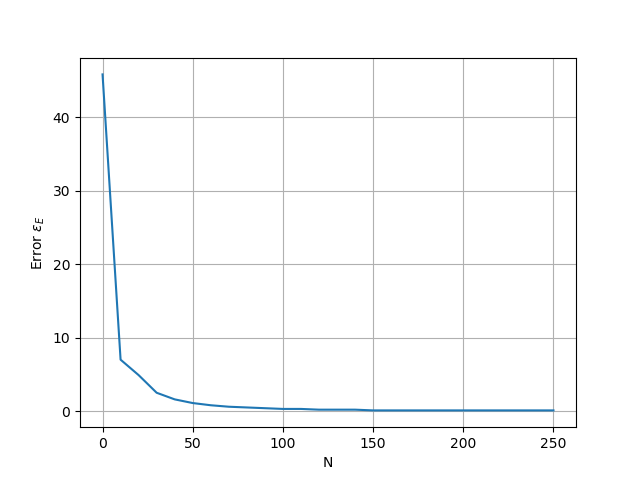
\includegraphics[scale=0.6]{fig1.png}
\caption{Plot of error for ten lowest energy values.}
\label{part 2: plot 1}
\end{figure}
Now adding a table of the three lowest energy values in a table for three chosen $N$ values, $E_J$ are computed energy values by Jacobi algorithm, while $E$ refers to the analytical values and are given in another table just below.
\begin{table}[H]
\center
\begin{tabular}{|c | c | c | c |}
\hline
N & 10 & 30 & 110\\
\hline
$E_J$ & $\begin{pmatrix} 1.343\\3.057\\5.529 \end{pmatrix}$ & $\begin{pmatrix} 1.482\\3.411\\5.279 \end{pmatrix}$ & $\begin{pmatrix} 1.499\\3.494\\5.484 \end{pmatrix}$\\
\hline
\end{tabular}
\label{part2: table 2}
\end{table}

\begin{table}[H]
\center
\caption{Table of analytical energy values $E$}
\begin{tabular}{| c | c | c | c |}
\hline
$E$ & 1.5 & 3.5 & 5.5\\
\hline 
\end{tabular}
\label{part 2: table 3}
\end{table}

Now lowering the approximation of infinity by changing $\rho_N=5$.
Adding plot of both results of error with $\rho_N=10$ as well
\begin{figure}[H]
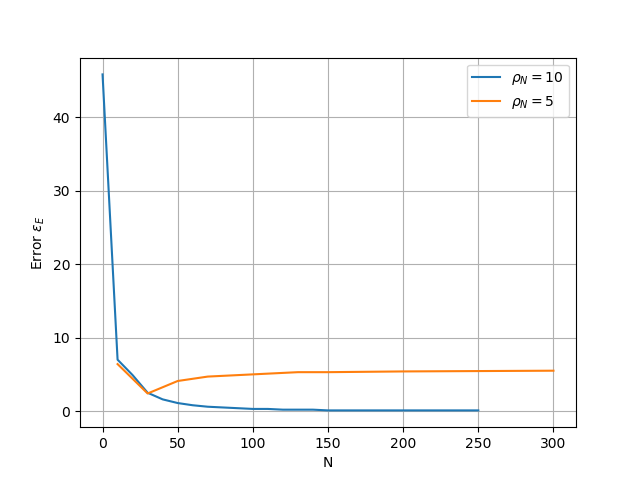
\includegraphics[scale=0.6]{fig2.png}
\center
\caption{Plot of error $\epsilon_N$ as function of number of computed eigenvalues $N$ for $\rho_N \in {5,10}$.}
\label{part2: plot 2}
\end{figure}

\subsection{Part 3: Schrodinger equation, Quantum dots}
Since we're only focusing on the ground state, we present a table of the computation results for the eigenvalues of varying potential strength $\omega_r$ with corresponding eigenvalue for the ground state $\lambda_0$. Keeping $\rho_N = 10$.

\begin{table}[H]
\center
\caption{Table showing eigenvalues for ground state $\lambda_0$ with corresponding potential strength $\omega_0$. For $N=100$ eigenvalue calculation in the Jacobi algorithm.}
\begin{tabular}{|c | c |}
\hline
$\omega_r$ & $ \lambda_0$\\
\hline
0.1 & 0.3 \\
\hline
0.5 & 2.2\\
\hline
1.0 & 4.1\\
\hline
5.0 & 17.4\\
\hline
\end{tabular}
\label{part 3: table 1}
\end{table}

\begin{figure}[H]
\center
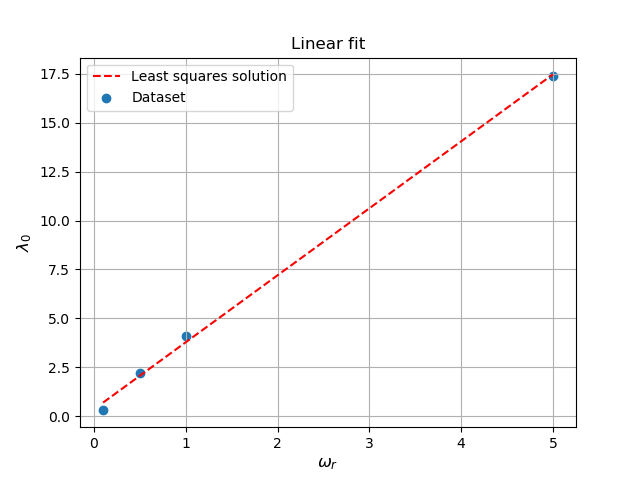
\includegraphics[scale=0.5]{lsqfit.png}
\caption{Least squares fit of $\lambda_0$ as function of $\omega_r$.}
\label{part 3: plot 5}
\end{figure}

Now extracting eigenvector containing $u_i$ corresponding to eigenvalue and plotting as a function of $\rho_i$

\begin{figure}[H]
\center
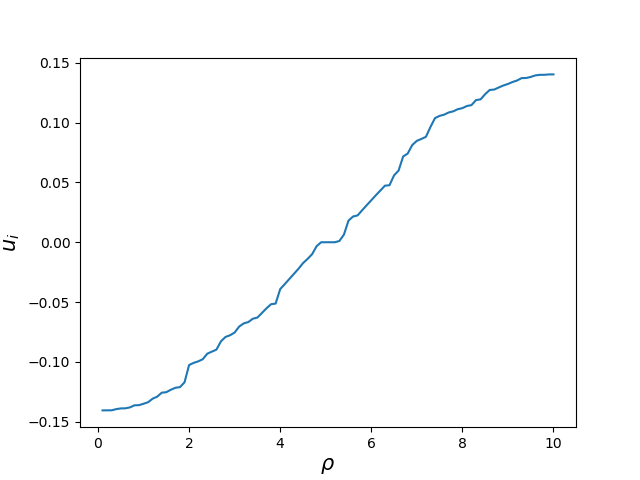
\includegraphics[scale=0.5]{wr001.png}
\caption{Plot of eigenvector corresponding to ground state $\lambda_0=0.3$ with oscillator potential $\omega_r = 0.1$.}
\label{part 3: plot 1}
\end{figure}

\begin{figure}[H]
\center
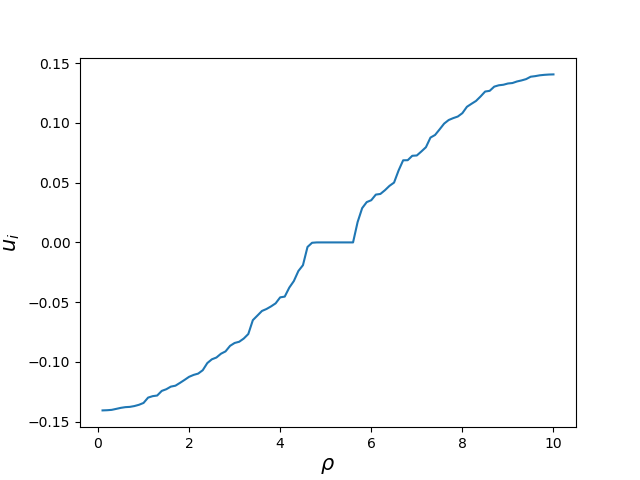
\includegraphics[scale=0.5]{wr05.png}
\caption{Plot of eigenvector corresponding to ground state $\lambda_0=2.2$ with oscillator potential $\omega_r = 0.5$.}
\label{part 3: plot 2}
\end{figure}

\begin{figure}[H]
\center
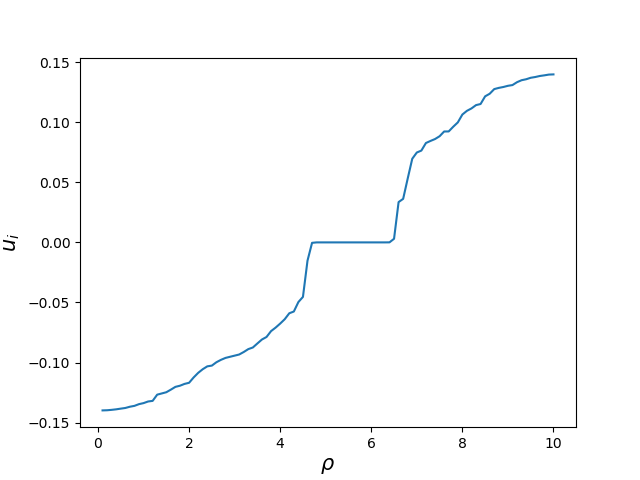
\includegraphics[scale=0.5]{wr1.png}
\caption{Plot of eigenvector corresponding to ground state $\lambda_0=4.1$ with oscillator potential $\omega_r = 1.0$.}
\label{part 3: plot 3}
\end{figure}

\begin{figure}[H]
\center
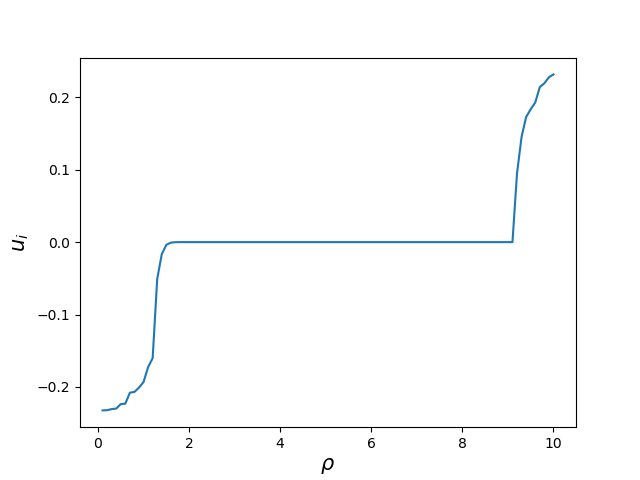
\includegraphics[scale=0.5]{wr5.png}
\caption{Plot of eigenvector corresponding to ground state $\lambda_0=17.4$ with oscillator potential $\omega_r = 5.0$.}
\label{part 3: plot 4}
\end{figure}

\section{Discussion}
From table (\ref{part1: table 1}) we see that the eigenvalues correspond to the fixed tolerance, although the computation times as seen in table (\ref{part 1: table 2}) seem to be in favour of the Jacobi algorithm. Dividing the mean values we can show that according to these computations, the written Jacobi algorithm runs about 17 times faster than numpy's linalg.eig function.\par
What was also observed when running the Jacobi algorithm several times was that our number of rotations function $R_{rot}$ (\ref{numberofRotequation}) was much better approximating the number of required rotations if changed to
\begin{equation}
N_{rot}(N)=2 N(N-1)
\end{equation}
namely that every non diagonal element must be zeroed out twice.\par
In part 2 many test runs with variations of the tolerances for the orthogonal conservation $\epsilon_V$ and the zero tolerance for the off diagonal elements of $A$ $\epsilon_J$ had to be testet in order for the energy values to be returned as sensible values. Thus having to decrease $\epsilon_V$ for increasing $N$ seems to be a natural consequence of floating point operations. Since the Jacobi algorithm keeps zeroing out non diagonal elements and rewriting earlier zeroed out non diagonals with new number which contain errors. Accumulating more and more errors for each rotation. \par
Moving on, we can see that $\rho_N=10$ was a presumably good approximation for infinity in the quantum case. In plot (\ref{part 2: plot 1}) we see the error in the first ten energy eigenvalues decrease rapidly with increasing $N$. It might not be a bad suggestion that the error goes as $\frac{1}{N}$ or even $\frac{1}{\sqrt{N}}$. A comment to table (\ref{part 2: table 1}) when it comes to the error at $N=300$. Due to the choice of significant digits this became rounded to zero, but it is (perhaps obviously) not exactly zero. So we shall interpret this as meaning practically zero. In other words, the accuracy of the eigenvalue computation increases with increasing N. If we consider the other much lower approximation to infinity we made, $\rho_N=5$, we can consider ($\ref{part2: plot 2}$), here the error starts out lower than for $\rho_N=10$, reaches a minima at around $N=30$, then increases very slowly (logarithmic perhaps) with increasing N. This might be explained by the fact that when $\rho_N$ increases, the step size decreases. Which should give a more accurate solution, while a lower $\rho_N$ tends to the opposite.\par
Finally in part 3, an analytical solution for the energy values were not available. So the computed eigenvalues have to be assumed correct or at least decent approximations. Table (\ref{part 3: table 1}) shows an increasing eigenvalue for an increasing $\omega_r$ (harmonic oscillator potential strength). Since the computed eigenvalues are proportional to the energy eigenvalues of the system, it means that there is also an increase in the hamiltonian (total) energy of the system with an increased potential strength. This makes sense since the electrons are, i.e given more energy when the potential strength is increased. In the same way you're applying more potential energy (thereby increasing total energy) to yourself when you move up a hill. The least squares fit in (\ref{part 3: plot 5}) suggests a proportionality constant of 3.5 between the computed eigenvalues for the ground state $\lambda_0$ and $\omega_r$. The plots (\ref{part 3: plot 1}) - (\ref{part 3: plot 4}) of the eigenstates show how the electrons have practically zero chance of existing in the center of the potential. The center in a physical sense would contain the cause of the potential, for instance protons. In this way we can interpret the increase in zero probability area which becomes very visible in plot (\ref{part 3: plot 4}) as an increase in the central charge, forcing the electrons to be more seperated.


\section{Concluding remarks}
By scaling differential equations, a common solver can be applied to several physical systems. For the particular systems we have found: writing a solver for the Jacobi algorithm in c++ may reduce runtime significantly when compared with other solvers. We've confirmed that this holds true for the numpy.linalg.eig eigenvalue solver. In part 2 we've found that a decent approximation to infinity for a quantum system is $\rho_N=10$, resulting in a difference in numerical and analytical energy values which approaches zero for relatively large values of N. Although other untested choices of $\rho_N$ might lead to better results.
\par
In part 3 we've found that increasing the potential strength in a 2 particle quantum systems leads to a proportional increase of energy with a proportionality constant of 3.5.
\section{Github-Repository}
\url{https://github.com/nhofield/fys3150Projects.git}

\section{\label{Referances} References}
\begin{itemize}
\item \url{http://compphysics.github.io/ComputationalPhysics/doc/Projects/2018/Project2/pdf/Project2.pdf}
\item \url{http://math.ecnu.edu.cn/~jypan/Teaching/books/2013%20Matrix%20Computations%204th.pdf}%
\end{itemize}

\end{document}
%
% ****** End of file aipsamp.tex ******